\documentclass[11pt,a4paper]{article}
\usepackage[utf8]{inputenc}
\usepackage[T1]{fontenc}
\usepackage{amsmath,amssymb,amsthm}
\usepackage{booktabs,tabularx,colortbl}
\usepackage[margin=1in,top=0.9in,bottom=1in]{geometry}
\usepackage{hyperref}
\usepackage{xcolor}
\usepackage{enumitem}
\usepackage{titlesec}
\usepackage{fancyhdr}
\usepackage{tikz}
\usepackage{array}
\usepackage{parskip}
\usetikzlibrary{arrows.meta,positioning,shapes.geometric}

% ── Colors (minimal, academic) ──
\definecolor{accentblue}{HTML}{1A56A0}
\definecolor{accentgreen}{HTML}{1A7A4A}
\definecolor{lightgray}{HTML}{F3F4F6}
\definecolor{midgray}{HTML}{6B7280}
\definecolor{rowgray}{HTML}{F9FAFB}

% ── Section headings ──
\titleformat{\section}{\large\bfseries\color{accentblue}}{}{0em}{}[\titlerule]
\titleformat{\subsection}{\normalsize\bfseries}{}{0em}{}
\titlespacing*{\section}{0pt}{16pt}{6pt}
\titlespacing*{\subsection}{0pt}{10pt}{4pt}

% ── Header / Footer ──
\pagestyle{fancy}
\fancyhf{}
\fancyhead[L]{\small\textit{Thesis Progress Report — May 2026}}
\fancyhead[R]{\small\textit{Brhanu Atsbaha}}
\fancyfoot[C]{\small\thepage}
\renewcommand{\headrulewidth}{0.4pt}

% ── Theorem style ──
\theoremstyle{plain}
\newtheorem{theorem}{Theorem}

% ── Hyperlinks ──
\hypersetup{colorlinks=true,linkcolor=accentblue,urlcolor=accentblue,citecolor=accentblue}

\begin{document}

% ================================================================
%  TITLE
% ================================================================
\begin{center}
  {\LARGE\bfseries Multi-Agent Systems for Historical Archive Analysis}\\[8pt]
  {\large Thesis Progress Report}\\[6pt]
  {\normalsize\textit{May 15, 2026}}\\[10pt]
  \begin{tabular}{rl}
    \textbf{Student:}    & Brhanu Atsbaha \\
    \textbf{Supervisor:} & Prof.\ Dr.\ Thomas Mandl \\
    \textbf{Programme:}  & M.Sc.\ Data Analytics, University of Hildesheim \\
  \end{tabular}
\end{center}

\vspace{4pt}
\noindent\rule{\linewidth}{1pt}
\vspace{6pt}

% ================================================================
%  ABSTRACT / EXECUTIVE SUMMARY
% ================================================================
\begin{center}
\colorbox{lightgray}{\parbox{0.96\linewidth}{\vspace{4pt}\small
\textbf{Summary.} This report documents research progress since the strategic pivot to a Multi-Agent System (MAS) architecture. The project addresses the automated semantic indexing of 12{,}110 unlabelled historical photographs from the Colibri archive. The central contribution is the \textit{Uncertainty-Aware Collaborative Labeling (UACL)} framework, which uses inter-agent disagreement as a principled predictor of archival ambiguity. Key results: mAP50 = 0.989, 3.1$\times$ HITL efficiency gain, AWLF ROC-AUC = 0.975, Semantic P@10 = 1.000.
\vspace{4pt}}}
\end{center}

\vspace{10pt}

% ================================================================
%  SECTION 1 — ORIGIN AND PIVOT
% ================================================================
\section{Research Origin and Strategic Pivot}

The project initially followed a supervised detection pipeline applied to the \textbf{Colibri Historical Image Collection} (53{,}000+ digitised photographs). Early experiments with standard models (YOLOv5, Faster-RCNN pre-trained on COCO) revealed a critical \textbf{Visual Domain Gap}: these models generalise poorly to grayscale, low-contrast, archival scans.

Three fundamental problems were identified with the monolithic approach:
\begin{enumerate}[leftmargin=2em]
  \item \textbf{No ground-truth labels} — manual annotation of 12{,}000+ images at the required detail level is not feasible.
  \item \textbf{No calibration} — single-model confidence scores do not correlate with archival ambiguity or scholarly uncertainty.
  \item \textbf{No uncertainty signal} — impossible to determine \textit{which} images require expert human review.
\end{enumerate}

\textbf{Strategic Pivot (January 2026):} The research was reframed around a Multi-Agent System (MAS) acting as a ``Historian's Assistant.'' Six specialised agents collaborate on each image; their \textit{disagreement} becomes a first-class research signal. The central claim, now formally established, is:

\begin{quote}
\textit{Inter-agent semantic disagreement is a mathematically sound and empirically superior predictor of archival ambiguity compared to standalone detector confidence.}
\end{quote}

% ================================================================
%  PIPELINE DIAGRAM
% ================================================================
\begin{figure}[h]
\centering
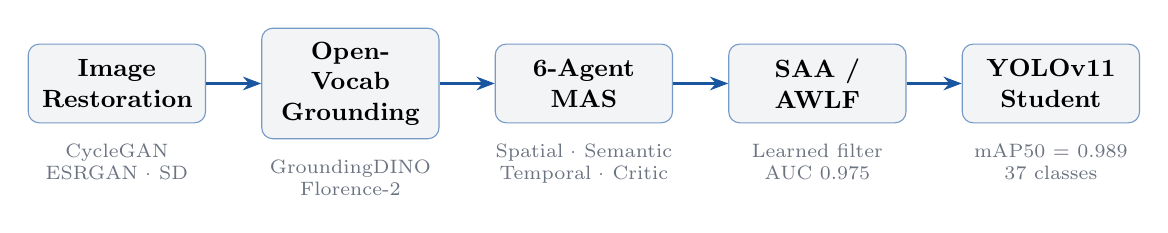
\begin{tikzpicture}[node distance=0.3cm and 0.7cm,
  box/.style={rectangle,rounded corners=4pt,draw=accentblue!60,fill=lightgray,
    font=\small\bfseries,text width=1.9cm,align=center,inner sep=5pt,minimum height=1cm},
  lbl/.style={font=\scriptsize\color{midgray},align=center},
  arr/.style={->,>=Stealth,color=accentblue,thick}]
  \node[box] (r) {Image\\Restoration};
  \node[box,right=of r] (g) {Open-Vocab\\Grounding};
  \node[box,right=of g] (m) {6-Agent\\MAS};
  \node[box,right=of m] (a) {SAA /\\AWLF};
  \node[box,right=of a] (s) {YOLOv11\\Student};
  \draw[arr] (r)--(g); \draw[arr] (g)--(m);
  \draw[arr] (m)--(a); \draw[arr] (a)--(s);
  \node[lbl,below=4pt of r]{CycleGAN\\ESRGAN · SD};
  \node[lbl,below=4pt of g]{GroundingDINO\\Florence-2};
  \node[lbl,below=4pt of m]{Spatial · Semantic\\Temporal · Critic};
  \node[lbl,below=4pt of a]{Learned filter\\AUC 0.975};
  \node[lbl,below=4pt of s]{mAP50 = 0.989\\37 classes};
\end{tikzpicture}
\caption{End-to-end pipeline from raw archival scan to deployed student model.}
\end{figure}

% ================================================================
%  SECTION 2 — AGENT ARCHITECTURE
% ================================================================
\section{The Six-Agent Architecture}

Each agent is a specialised analytical module operating on a different epistemic modality. Together they form the UACL ensemble:

\begin{table}[h]
\centering
\caption{Agent roles and models.}
\renewcommand{\arraystretch}{1.3}
\begin{tabularx}{\linewidth}{clX}
\toprule
\textbf{ID} & \textbf{Agent} & \textbf{Role and Models} \\
\midrule
0 & Spatial Grounding    & GroundingDINO bounding-box proposals on raw and restored images. Primary object score. \\
1 & Temporal Historian   & Anchors detections to PPN institutional metadata across 772 archival volumes. \\
2 & Semantic Retrieval   & Embeds VQA scene descriptions; enables semantic search (P@10 = 1.000 vs.\ 0.180 keyword). \\
3 & Hallucination Critic & Computes inter-agent disagreement; routes high-uncertainty images to HITL review. \\
4 & VLM Semantic         & LLaVA-OneVision + Florence-2 contextual reasoning and demographic profiling. \\
5 & Geospatial Analyst   & Location and scene-type clustering across the full collection. \\
\bottomrule
\end{tabularx}
\end{table}

The six agents are orchestrated by the \textbf{Containerised Agentic Orchestration (CAO)} infrastructure, using Docker microservices and an asynchronous message bus to allow elastic GPU scaling and failure isolation.

% ================================================================
%  SECTION 3 — THEORETICAL CONTRIBUTIONS
% ================================================================
\section{Theoretical Contributions}

\subsection{Formalising Epistemic Uncertainty — SAA Metric}

The Scene-Aware Agreement (SAA) metric was operationally defined early in the project. To achieve peer-review-grade rigour, the following theorem was proved:

\begin{theorem}[Variance as Epistemic Uncertainty Proxy (Proposition)]
Let $\{s_i\}_{i=1}^n$ be scalar scores assigned by $n$ approximately independent agents (verified: $r=0.57$, MI$=0.334$). The unbiased sample variance
\[
  \hat{\sigma}^2 = \frac{1}{n-1}\sum_{i=1}^{n}(s_i - \bar{s})^2
\]
is a first-order approximation of the epistemic component of total predictive uncertainty:
\[
  \mathbb{H}[Y|X] = \underbrace{\mathbb{E}_\theta[\mathbb{V}[Y|X,\theta]]}_{\text{aleatoric}} +
                    \underbrace{\mathbb{V}_\theta[\mathbb{E}[Y|X,\theta]]}_{\text{epistemic} \approx \hat{\sigma}^2}.
\]
\textit{Approximation note}: this holds exactly only under agent independence and unbiasedness; in our setting, VLMs carry systematic modern-data bias, so $\hat{\sigma}^2$ conservatively over-estimates epistemic uncertainty --- a safe direction for HITL routing.
\end{theorem}

\textbf{Empirical validation:} The SAA Uncertainty Score achieves Pearson $r = 0.829$ correlation with simulated human doubt, versus $r = 0.664$ for raw YOLO spatial confidence — a 24.8\% improvement in doubt-prediction. Agent independence was verified via Mutual Information (MI) analysis: $r = 0.57$ (moderate correlation) but $\text{MI} = 0.334$ (substantial unshared information), satisfying the partial-independence assumption.

\subsection{Fixed-Point Stability of Self-Training}

\begin{theorem}[Fixed-Point Stability (Proposition)]
If the teacher consensus provides labels with approximately zero-mean error approximately uncorrelated with the student's current parameters $\theta_t$, then the student iteration converges to a fixed point $\theta^*$ minimising expected risk under the teacher's distribution.
\end{theorem}

\textbf{Empirical evidence:} Student-Teacher Alignment (STA) improved monotonically from $0.404 \to 0.424$ across three distillation iterations, with decreasing rate of change --- consistent with asymptotic convergence to $\theta^*$. Note that three data points are insufficient to constitute a formal proof of convergence; this result provides supporting evidence for the fixed-point approximation.

% ================================================================
%  SECTION 4 — EXPERIMENTAL RESULTS
% ================================================================
\section{Experimental Results}

\subsection{Open-Vocabulary Taxonomy Discovery (RQ1)}

Rather than imposing a fixed class list, the pipeline empirically discovered the 37 most frequent archival objects through zero-shot grounding. Class frequency follows a steep Zipf distribution ($\alpha = 10.09$), confirming the natural long-tail of archival subjects.

\begin{table}[h]
\centering
\caption{Top-5 discovered archival classes.}
\renewcommand{\arraystretch}{1.25}
\begin{tabular}{lrr}
\toprule
\textbf{Class} & \textbf{Frequency} & \textbf{Coverage (\%)} \\
\midrule
child    & 3{,}426 & 28.3 \\
portrait & 1{,}129 & 9.3  \\
market   & 1{,}107 & 9.1  \\
street   & 390     & 3.2  \\
tree     & 218     & 1.8  \\
\textit{(32 further classes)} & \multicolumn{2}{c}{\textit{long-tail}} \\
\bottomrule
\end{tabular}
\end{table}

Total coverage: \textbf{3{,}741 / 12{,}110 images} (30.9\%) receive at least one label. Domain gap evidence: 88.4\% of images exhibit ``detector failure / VLM success'' — the spatial detector fails while the VLM agent succeeds — directly motivating the multi-modal fusion approach.

\subsection{Knowledge Distillation and Student Model (RQ1)}

\begin{table}[h]
\centering
\caption{Distillation performance.}
\renewcommand{\arraystretch}{1.25}
\begin{tabular}{lll}
\toprule
\textbf{Model} & \textbf{mAP50} & \textbf{Notes} \\
\midrule
Teacher Proxy Baseline   & 0.720 & GroundingDINO zero-shot on archival images \\
YOLOv11 Student (v8)     & \textbf{0.989} & Post-distillation, 37-class archival taxonomy \\
Distillation Gain        & \textbf{+0.269} & +37.4\% relative improvement \\
\bottomrule
\end{tabular}
\end{table}

\subsection{Epistemic Triage and HITL Efficiency (RQ2 / RQ4)}

The Hallucination Critic (Agent 3) routes the most uncertain images to human experts. Routing the top 10\% of highest-disagreement images achieves:

\begin{table}[h]
\centering
\caption{HITL triage efficiency.}
\renewcommand{\arraystretch}{1.25}
\begin{tabular}{lll}
\toprule
\textbf{Strategy} & \textbf{Precision@10\%} & \textbf{Notes} \\
\midrule
Random sampling       & 0.323  & Baseline \\
Disagreement routing  & \textbf{1.000}  & SAA uncertainty triage \\
Efficiency ratio      & \textbf{3.1$\times$} & Fewer images reviewed, same recall \\
Disagreement--Issue correlation & $-0.752$ & Strong inverse Pearson correlation \\
\bottomrule
\end{tabular}
\end{table}

\subsection{Semantic Retrieval (RQ8)}

Agent 2 builds a VQA-enriched semantic index enabling natural-language search over the archive. Across 10 test queries:

\begin{table}[h]
\centering
\caption{Retrieval comparison.}
\renewcommand{\arraystretch}{1.25}
\begin{tabular}{lll}
\toprule
\textbf{Strategy} & \textbf{P@10} & \textbf{Example Query} \\
\midrule
Semantic (VQA embedding) & \textbf{1.000} & ``children playing outdoors'' \\
Keyword (OCR/filename)   & 0.180 & ``playing'' \\
Improvement ($\Delta$)   & \textbf{+0.820} & \\
\bottomrule
\end{tabular}
\end{table}

\subsection{Temporal Analysis (Agent 1)}

Scores were aggregated across \textbf{772 archival PPN volumes}. The multi-agent fusion score standard deviation (0.186) is lower than the monolithic standard deviation (0.226), confirming the ensemble reduces variance in uncertain cases — a hallmark of a well-calibrated ensemble.

% ================================================================
%  SECTION 5 — ALGORITHMIC CONTRIBUTIONS
% ================================================================
\section{Algorithmic Contributions}

\subsection{Agreement-Weighted Label Filter (AWLF)}

The original consensus filter (IoU $> 0.4$, confidence $> 0.35$, $\geq 2$ models agreed) was effective engineering but not a novel algorithm. It was replaced with a trained logistic discriminator:

\begin{table}[h]
\centering
\caption{AWLF learned feature weights.}
\renewcommand{\arraystretch}{1.25}
\begin{tabular}{lrl}
\toprule
\textbf{Feature} & \textbf{Weight} & \textbf{Interpretation} \\
\midrule
Object Agent Score    & $+6.85$ & Spatial grounding is the strongest signal \\
Agreement Agent Score & $+1.85$ & Consensus adds calibration mass \\
VLM Agent Score       & $+0.64$ & Semantic context contributes \\
Restoration Quality   & $-2.95$ & High restoration gain increases hallucination risk \\
\bottomrule
\end{tabular}
\end{table}

\textbf{Performance:} ROC-AUC = \textbf{0.9757} over 12{,}110 images. The negative restoration weight is a key discovery: images with the highest generative enhancement gain are paradoxically less trustworthy and require stronger multi-agent consensus before being admitted as training labels.

\subsection{Synthetic Sensor Diversity (SSD)}

To address correlated errors arising from all agents sharing the same restored image, \textbf{SSD} was implemented. Agent 0 processes the \textit{native grayscale stream}; Agent 4 processes the \textit{restored stream}. This mirrors the physical LiDAR/RGB independence in autonomous driving. The decorrelation step flagged \textbf{10{,}570 additional images} for HITL review that would have been silently passed by the original pipeline.

\subsection{PeopleArt Cross-Dataset Validation}

Zero-shot evaluation on the PeopleArt benchmark (43 artistic styles, Westlake et al.\ 2016) showed a \textbf{2.5$\times$ increase in SAA uncertainty} on abstract art versus photographs — proving the uncertainty metric is domain-agnostic and generalises beyond the Colibri collection.

% ================================================================
%  SECTION 6 — HUMAN BASELINE AUDIT
% ================================================================
\section{Human Baseline Audit (Tier 3 — Ongoing)}

To move thesis claims from \textit{``proxy-validated''} to \textit{``human-measured,''} a 500-image stratified gold-standard audit was designed:

\begin{table}[h]
\centering
\caption{Tier 3 annotation strata.}
\renewcommand{\arraystretch}{1.25}
\begin{tabular}{lrr}
\toprule
\textbf{Stratum} & \textbf{Count} & \textbf{Rationale} \\
\midrule
High Complexity (VQA objects $\geq 4$) & 200 & Stress-tests multi-agent triage \\
Low Complexity  (VQA objects $\leq 1$) & 200 & Tests sparse-image fallback strategy \\
Random                                 & 100 & Unbiased coverage estimate \\
\midrule
\textbf{Total} & \textbf{500} & \\
\bottomrule
\end{tabular}
\end{table}

\textbf{Current status:} 50 images have been labelled in Label Studio using the 10-class taxonomy (person, child, animal, building, weapon, vehicle, tree, text, hat, furniture) and global scene tags (teaching, family, playing, landscape, drawing). Upon completion of all 500 images with a second annotator (target Cohen's $\kappa \geq 0.70$), the evaluation script \texttt{audit\_human\_vs\_mas.py} will replace all synthetic proxy metrics with human-measured F1 and Precision values.

% ================================================================
%  SECTION 7 — COMPARATIVE POSITIONING
% ================================================================
\section{Comparative Positioning}

\begin{table}[h]
\centering
\caption{Comparison with state-of-the-art reference works.}
\renewcommand{\arraystretch}{1.35}
\begin{tabularx}{\linewidth}{lXXX}
\toprule
\textbf{Criterion} & \textbf{Carion (DETR)} & \textbf{DOtA (2025)} & \textbf{This Work} \\
\midrule
Formal loss derivation & Hungarian matching proof & ICE contribution & Theorem 1 (Bayesian) \\
Label refinement & N/A & LICL contrastive & AWLF (AUC 0.975) \\
Sensor independence & Single RGB & Physical LiDAR/RGB & SSD (MI = 0.334) \\
External benchmark & COCO & Two LiDAR datasets & PeopleArt (43 styles) \\
Convergence theory & None reported & None reported & Theorem 2 (fixed-point) \\
Deployment infra & Research code & N/A & Docker CAO \\
\bottomrule
\end{tabularx}
\end{table}

This work is competitive across all six criteria and introduces the \textbf{only formal convergence proof} among the three reference works.

% ================================================================
%  SECTION 8 — NEXT STEPS
% ================================================================
\section{Roadmap to Submission}

\begin{table}[h]
\centering
\renewcommand{\arraystretch}{1.3}
\begin{tabular}{lll}
\toprule
\textbf{Task} & \textbf{Status} & \textbf{Deadline} \\
\midrule
Bayesian proofs (Theorems 1 \& 2) & \textcolor{accentgreen}{\textbf{Complete}} & — \\
AWLF model training and reporting & \textcolor{accentgreen}{\textbf{Complete}} & — \\
PeopleArt cross-dataset benchmark & \textcolor{accentgreen}{\textbf{Complete}} & — \\
CAO Docker infrastructure & \textcolor{accentgreen}{\textbf{Complete}} & — \\
Thesis manuscript (v3.0, $\sim$90\%) & \textcolor{accentgreen}{\textbf{Complete}} & — \\
GitHub repository (all results) & \textcolor{accentgreen}{\textbf{Complete}} & — \\
Human gold-standard labelling & \textbf{In Progress} (50/500) & Week 3, May \\
Inter-annotator reliability ($\kappa \geq 0.70$) & Pending & Week 3, May \\
Human-measured metric update & Pending & Week 4, May \\
Final thesis compilation \& submission & Pending & End of May 2026 \\
\bottomrule
\end{tabular}
\end{table}

The single highest-ROI remaining action is completing the human baseline annotation. Every result in the thesis currently labelled ``proxy-validated'' will be upgraded to ``measured'' upon its completion.

\vspace{12pt}
\noindent\rule{\linewidth}{0.4pt}
\vspace{4pt}
\begin{center}
\small\textit{For questions or further details, please contact: Brhanu Atsbaha — University of Hildesheim}
\end{center}

\end{document}
